\section{应用与结论}

\begin{frame}{智能驾驶环境下多目标跟踪和分析系统——灵动慧眼}
	\begin{figure}[!t]
		\centering
		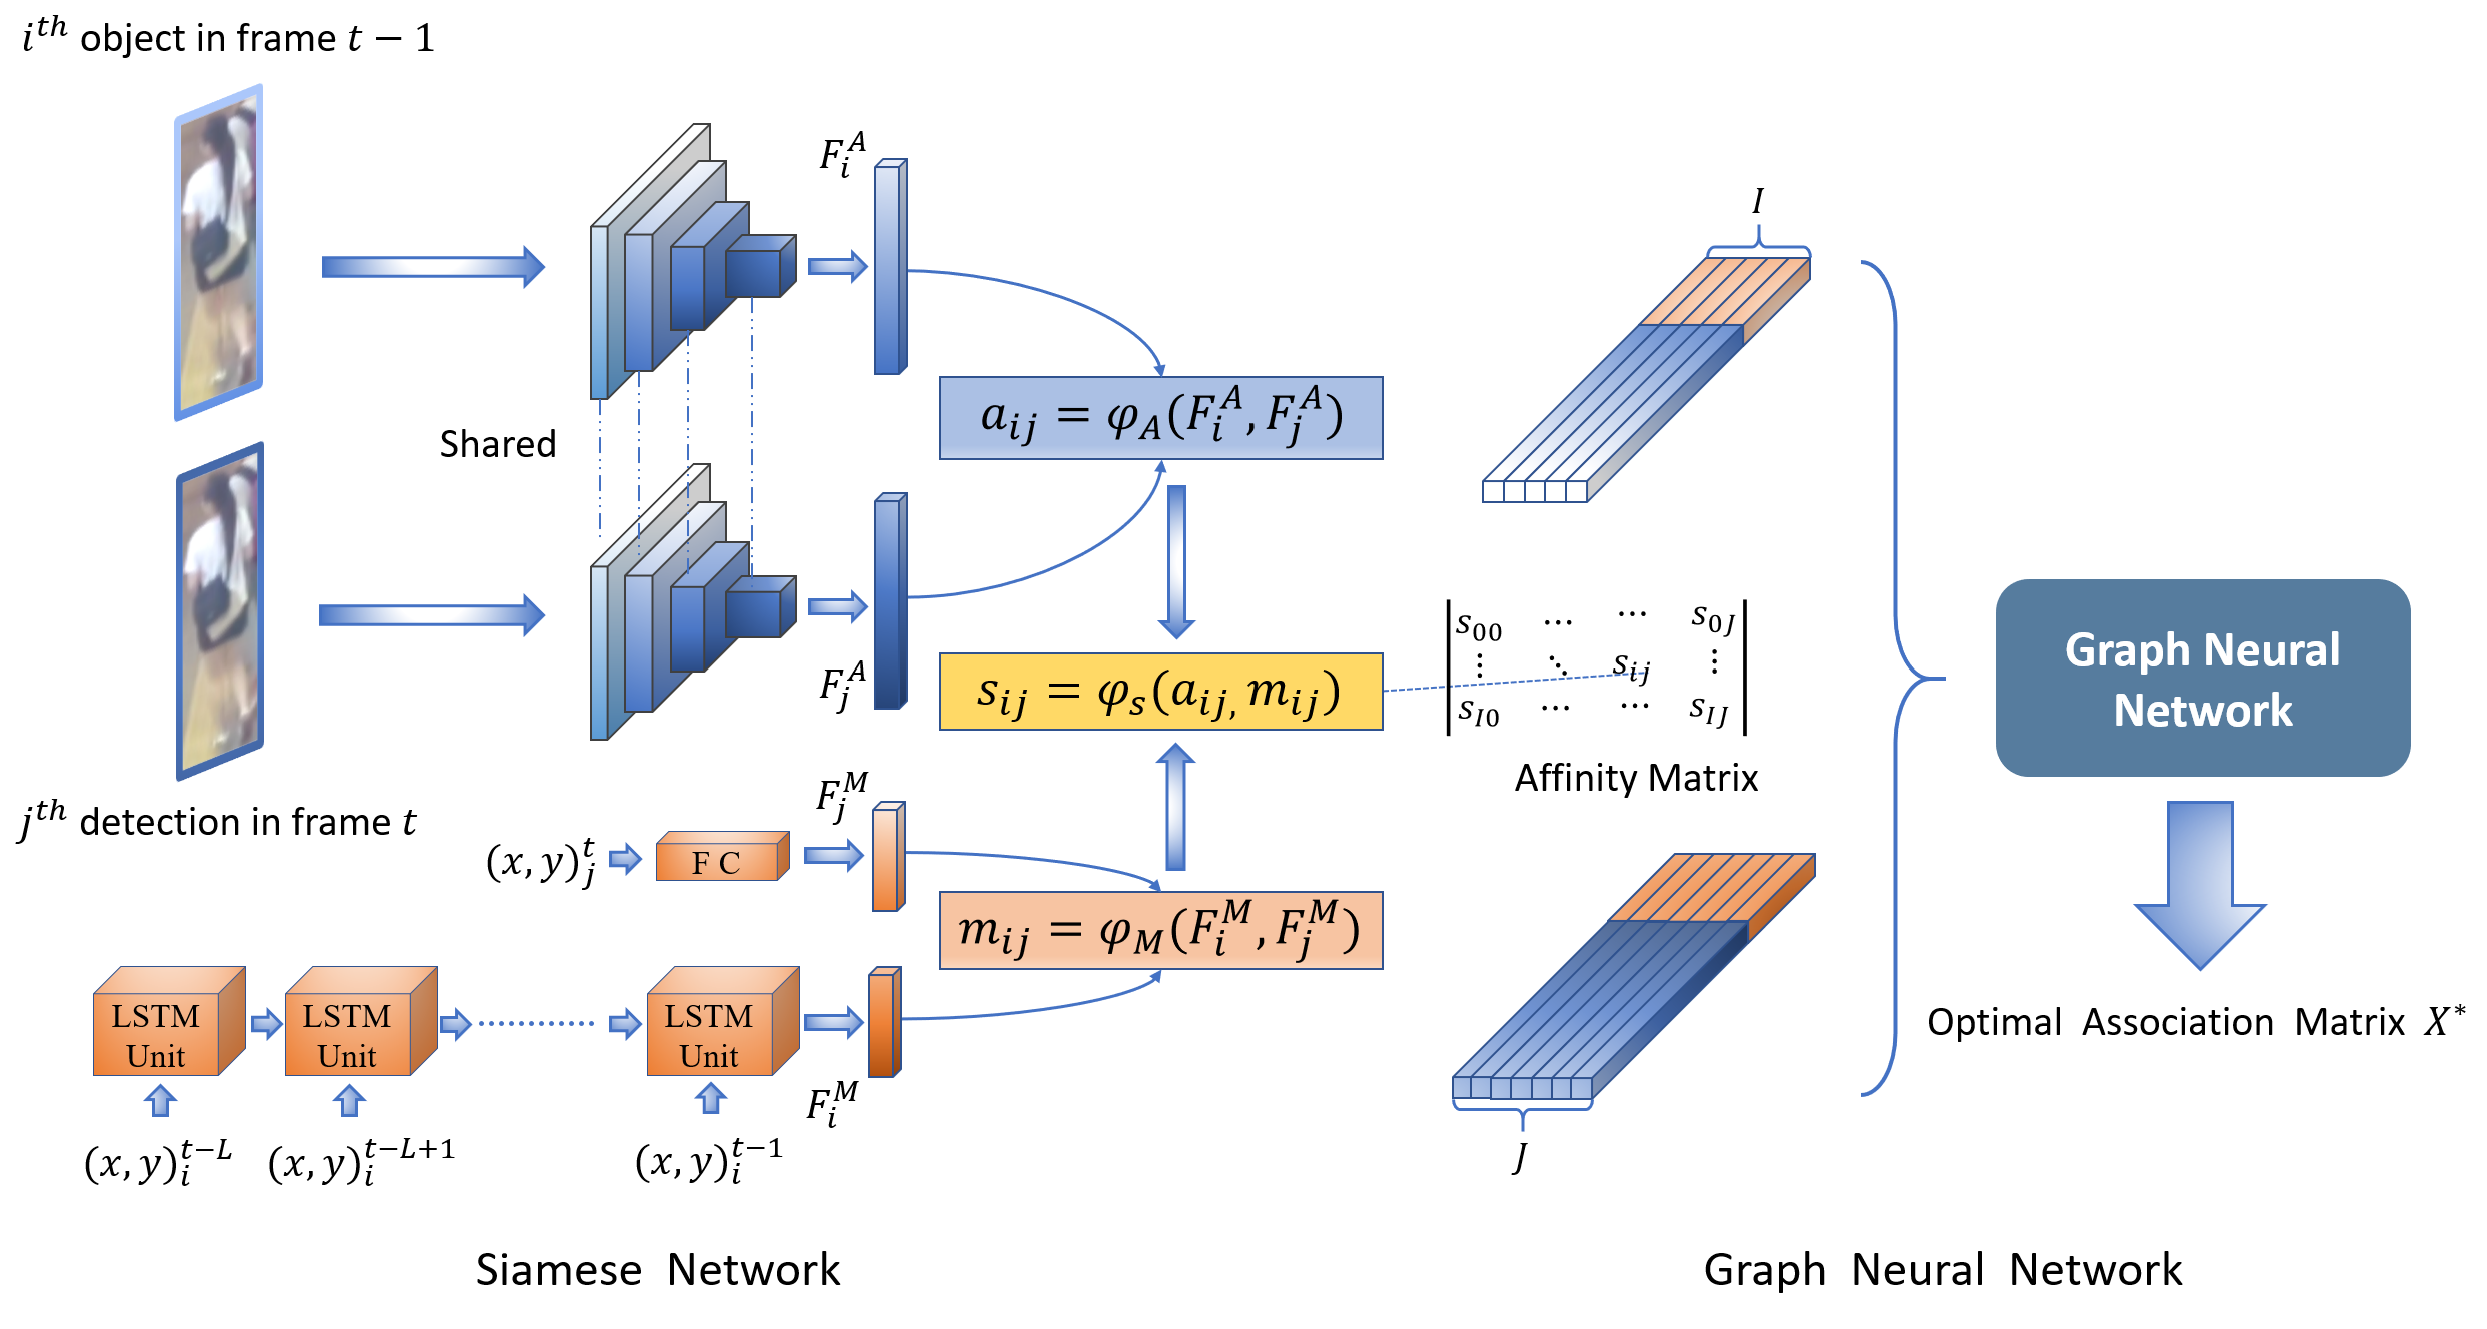
\includegraphics[width=4.5in]{../figures/C6Fig/pipeline.pdf}
		\caption{灵动慧眼系统的架构设计}
	\end{figure}
\end{frame}


\begin{frame}{智能驾驶环境下多目标跟踪和分析系统——灵动慧眼}
	\begin{figure}[!t]
		\centering
		\includegraphics[width=4.0in]{../figures/C6Fig/dongfanghong.pdf}
		\caption{复杂交通场景下的多目标跟踪和统计效果}
	\end{figure}
\end{frame}


\begin{frame}
	\frametitle{结论}
	\begin{block}{\textbf{本文主要贡献}}
		\begin{itemize}
			\item<0-> 提出了一种新的神经解剖对齐的类脑跟踪模型,以解决深度跟踪模型精度和人脑本身处理平稳跟踪机理之间的矛盾
			\item<0-> 提出了一种专注于跨时空范围的非局部注意力模型
			\item<0-> 提出了一种时空互表征学习方法
			\item<0-> 提出了一种端到端的模型和训练方法
		\end{itemize}
	\end{block}
	
	\begin{block}{\textbf{未来工作展望}}
		\begin{enumerate}
			\item<0-> 加入大脑皮层腹侧流类脑结构的设计,并考虑其它模态的融合
			\item<0-> 提高基于预测跟踪范式的运行效率
			\item<0-> 设计完全端到端检测跟踪模型和训练算法,并实现像素级跟踪
		\end{enumerate}
	\end{block}
\end{frame}

%\begin{frame}{结论}  %将来可做的方向
%	\begin{itemize}
%		\item<0-> Get more people to try this
%		\item<0-> Benchmark the entire system in the wild
%		\item<0-> Profit!
%	\end{itemize}
%\end{frame}

\begin{frame}
	\begin{center}
		\begin{minipage}{1\textwidth}
			\setbeamercolor{mybox}{fg=white, bg=black!50!blue}
			\begin{beamercolorbox}[wd=0.70\textwidth, rounded=true, shadow=true]{mybox}
				\LARGE \centering 谢谢!  %结束语
			\end{beamercolorbox}
		\end{minipage}
	\end{center}
\end{frame}

%\begin{frame}{Q\&A}
%	\begin{center}
%		\begin{minipage}{1\textwidth}
%			\setbeamercolor{mybox}{fg=white, bg=black!50!blue}
%			\begin{beamercolorbox}[wd=0.70\textwidth, rounded=true, shadow=true]{mybox}
%				\LARGE \centering  Questions?  %请求提问
%			\end{beamercolorbox}
%		\end{minipage}
%	\end{center}
%\end{frame}


% 参考文献太多,允许换页
\begin{frame}[allowframebreaks]{参考文献}
%	\bibliographystyle{apalike}
	\printbibliography
%	\bibliography{../reference.bib} % The file containing the bibliography
\end{frame}

%\begin{frame}{参考文献}
%	\printbibliography
%\end{frame}